%!TEX root = draft.tex
\section{Scaling} \label{sec:scaling}
In this section we present results that show the scalability of our algorithms. All of our tests have been run on the Stampede cluster at Texas Advanced Computing Center (TACC). Each node of Stampede has 2 eight-core Xenon E5-2680 processors clocked at 2.7 GHz with 32 GB of DDR3-1600 MHz memory and interconnected using an InfiniBand network. Unless explicitly mentioned otherwise, in all tests we use all 16 cores of every node. Finally, in all cases we report the maximum wall time recorded using PETSc's logging interface which has a temporal resolution of roughly $0.1 \: \mu s$.

\subsection{Interpolation}
In this section we show results for a simple test to measure the scalability of the interpolation algorithm \ref{alg:interpolation}. The test consists of interpolating a function at a number of random points on a randomly refined octree in three dimensions. We consider two cases. A small test on a level 9 tree with roughtly 20M cells and 33M nodes and larger test on a level 13 tree with roughly 128M cells and 280M nodes. In both cases number of randomly generated points are chosen to be equal to the number of nodes and the stablized second-order interpolation of \cite{Min;Gibou:07:A-second-order-accur} was performed 10 times to smooth out possible timing fluctuations.

To simulate the effect of different CFL numbers, we generate the random points such that on each processor $\alpha$ percentage of them are located outside the processor boundary and thus will initiate communication. Scaling results are presented for $\alpha = 5 \%$ and $\alpha = 95\%$ for both small and large problems in figure \ref{fig:interpolation}. Excellent scaling is obtained for the small problem for $P = 16-512$ even when $95\%$ of interpolation points are remote to processors. For the larger problem, communication overhead prevents further scaling of algorithm beyond $4096$ processors when $\alpha = 95\%$. Note that for $\alpha = 5\%$, even though some sections of algorithm stop scaling, the overall algorithm still scales since the local work dominates the timing. This illustrates the effectiveness of non-blocking communication pattern in algorithm \ref{alg:interpolation}.

\begin{figure}[htbp]
	\begin{center}
		\subfigure[$N_G = 33\times 10^6$, $\alpha = 5\%$]{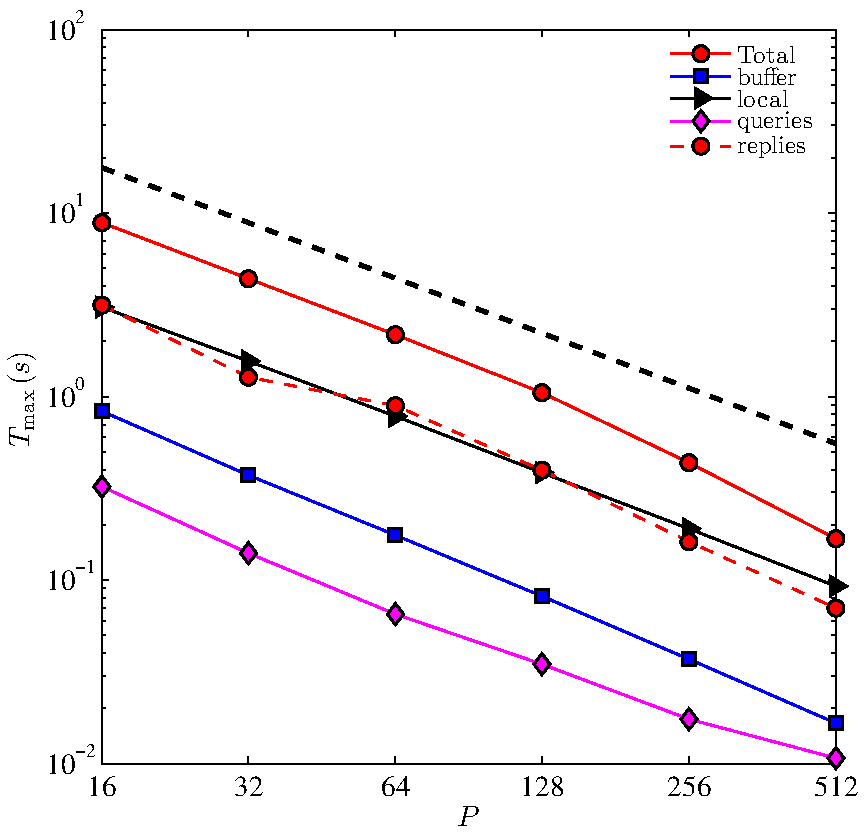
\includegraphics[width = 0.45 \textwidth] {figures/interpolation_small_05.pdf}}
		\subfigure[$N_G = 33\times 10^6$, $\alpha = 95\%$]{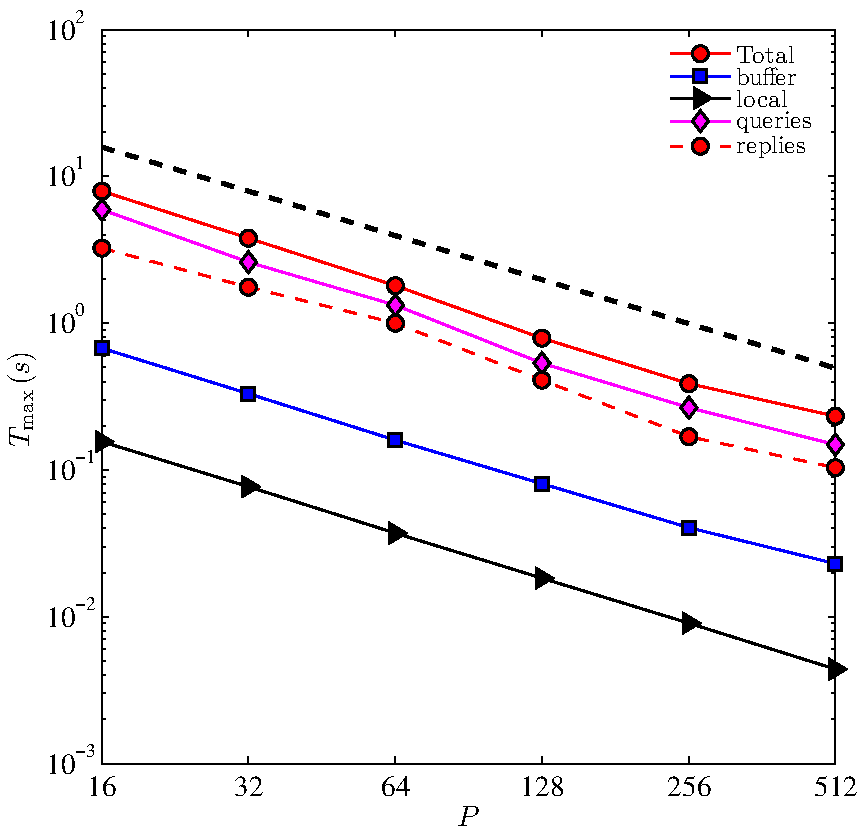
\includegraphics[width = 0.45 \textwidth] {figures/interpolation_small_95.pdf}}
		\\
		\subfigure[$N_G = 280\times 10^6$, $\alpha = 5\%$]{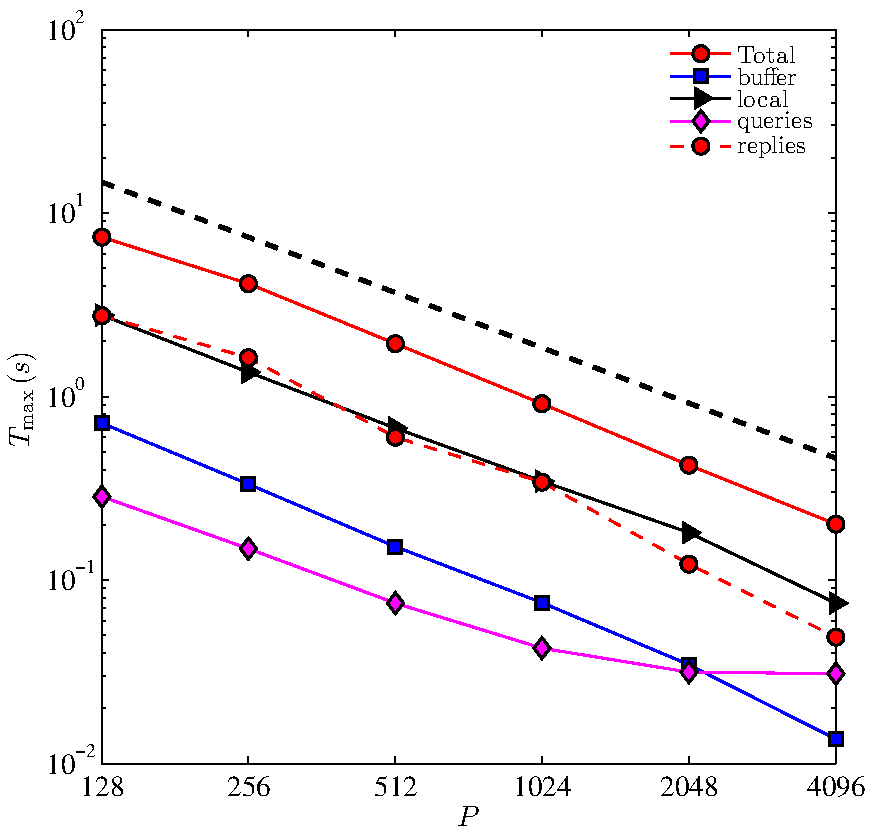
\includegraphics[width = 0.45 \textwidth] {figures/interpolation_large_05.pdf}}
		\subfigure[$N_G = 280\times 10^6$, $\alpha = 95\%$]{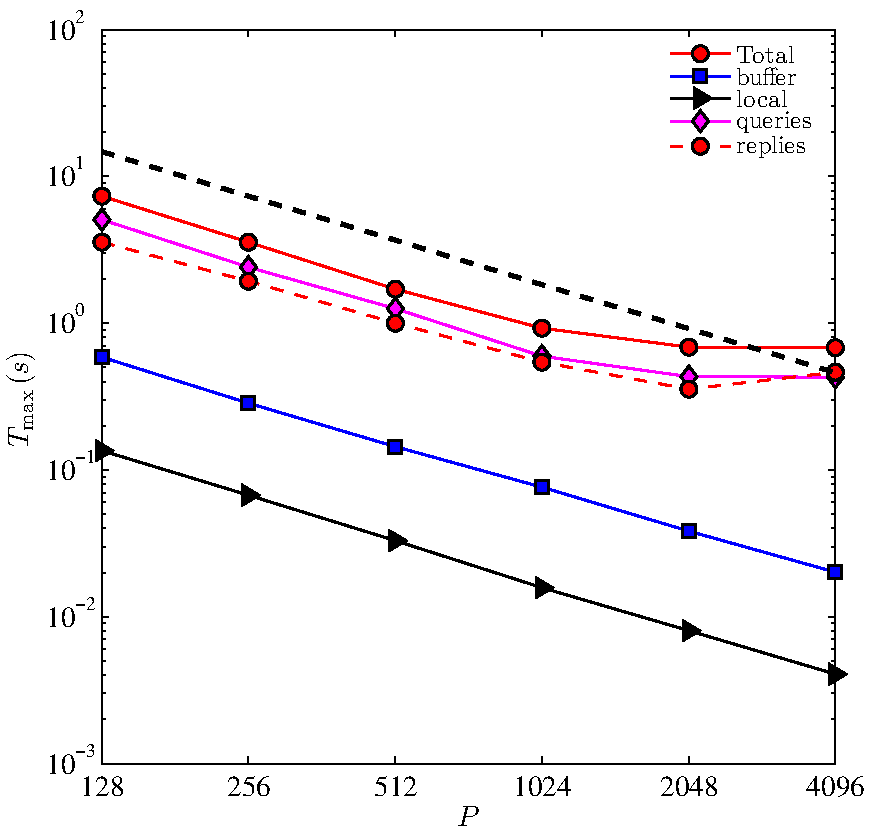
\includegraphics[width = 0.45 \textwidth] {figures/interpolation_large_95.pdf}}
	\end{center}
	\caption{Strong scaling of algorithm \ref{alg:interpolation} for several tests where $N_G$ denotes the number of random interpolation points (same as number of nodes in the octree) and $\alpha$ denotes the percentage of these points that are remote to each processor. Here ``Total'' represents the total time spent in the interpolation while ``buffer'', ``local'', ``queries'', and ``replies'' represent the the timing for different sections (c.f. algorithm \ref{alg:interpolation}). Results indicate excellent scaling for the small test (a-b) and for the large test when $\alpha = 5\%$ (c). For the extreme case (d) the algorithm stops scaling at $4096$ processors due to communication overhead.}
	\label{fig:interpolation}
\end{figure}

\subsection{Semi-Lagrangian}

% \subsection{Reinitialization} \label{section::scaling_reinitialization}

% The reinitialization procedure presented in section \ref{section::reinitialization} necessitates the second order derivatives of the level-set function for the second order discretization in space. The finite difference schemes we implemented rely on the description of the neighborhood of each vertex in the adaptive tree environment. This information can either be computed on the fly or stored in a buffer. Fetching the neighbors information is rather time consuming and was observed to improve the overall scalability of the algorithm by increasing the local computation load. However, it slowed down the procedure significantly and therefore we choose to present the buffered version of the implementation. If one was to be limited in memory, constructing the neighborhood information on the fly would be a desirable option and would lead to better scaling, but in our case memory is not a limiting factor.

% The scaling results are presented in figure \ref{fig::scaling_reinitialization} and demonstrate satisfying scalability. Taking for reference the timing with $128$ processes, we observe efficiencies of $0.877$ with $1024$ processes, $0.763$ with $2048$ processes and $0.609$ with $4096$ processes.

% \begin{figure}[ht!]
% \begin{center}
% 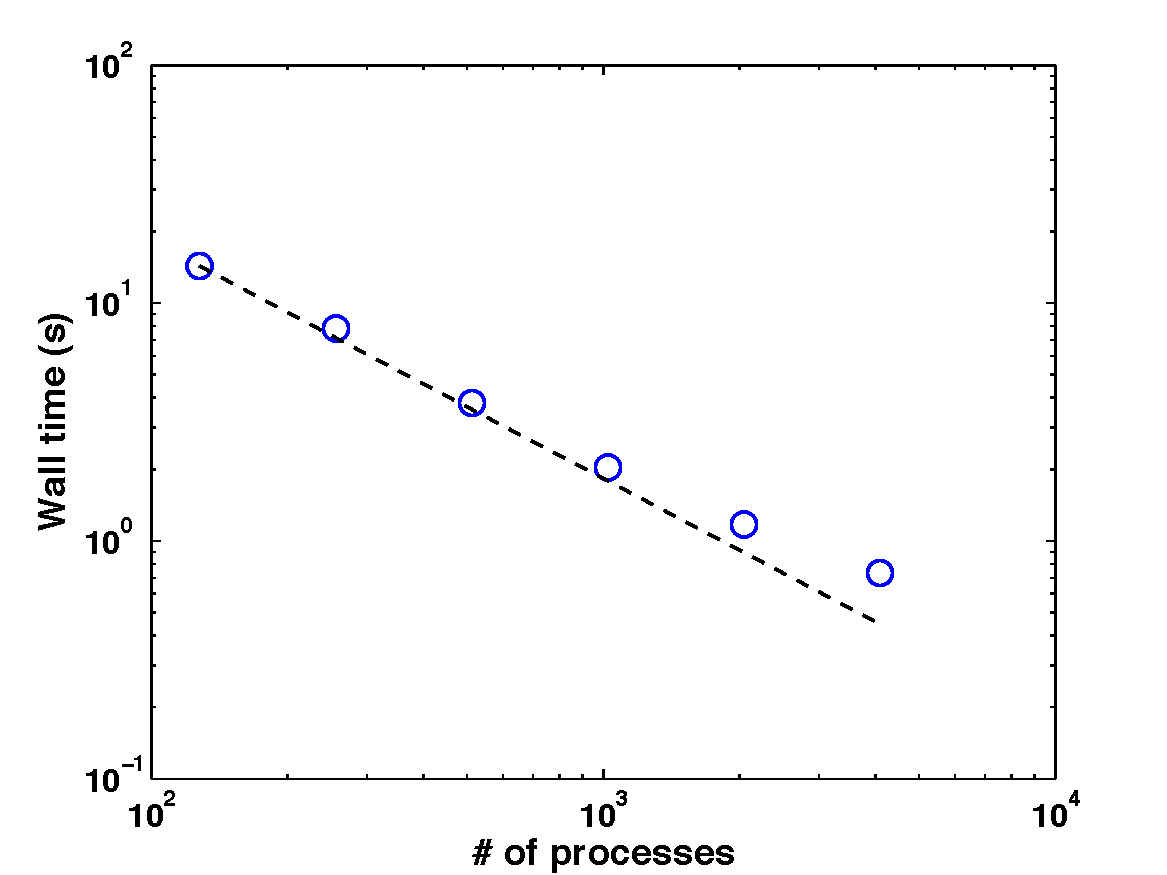
\includegraphics[width=.7\textwidth]{figures/scaling_reinitialization_1st_time_2nd_space_with_buffer.pdf}
% \caption{Scalability of the reinitialization procedure presented in section \ref{section::reinitialization} and analyzed in section \ref{section::scaling_reinitialization}.} \label{fig::scaling_reinitialization}
% \end{center}
% \end{figure}

% \subsection{Poisson solver}